\documentclass[t]{beamer}
\usetheme{Warsaw}
\usepackage{amsmath,amsthm,amssymb,hyperref,physics,mathtools,graphicx}

\newcommand{\ua}{\uparrow}
\newcommand{\da}{\downarrow}

\title{Quantum Spin}
\author{Dylan Mcintyre and Kenny Roffo}
\date{April 2, 2015}
\institute{SUNY Oswego}

\begin{document}

\frame{
\titlepage
}

\frame{
\frametitle{Classical Spin}
\begin{itemize}
\item Classically, a mass can exhibit two types of angular momentum - Orbital and Spin
\pause
\item Orbital momentum is momentum due to revolution, spin momentum is due to rotation
\pause
\item Spin momentum is really just the sum of the orbital momentum of all the particles which make up the object
\end{itemize}
}

\frame{
\frametitle{Quantum Spin}
\begin{itemize}
\item In Quantum Physics, we deal with elementary particles, and thus the spin momentum cannot be defined in the same manner
\pause
\item Instead we consider particles to have \emph{intrinsic} angular momentum, $\vb{S}$
\pause
\item Elementary Particles each have a specific spin which never changes
\pause
\item A few examples:
\end{itemize}
\begin{center}
\begin{tabular}{|c|c|}
\hline
Particle & Spin\\
\hline
pi meson & 0\\
\hline
$e^-,p,n$ & $\frac{1}{2}$\\
\hline
photon & 1\\
\hline
delta & $\frac{3}{2}$\\
\hline
graviton & 2\\
\hline
\end{tabular}
\end{center}
}

\frame{
\frametitle{Defining the Spin Operators}
\begin{itemize}
\item We begin with the commutation relations:
\begin{displaymath}
[S_x,S_y]=i\hbar S_z \text{\hspace{0.4in}} [S_y,S_z]=i\hbar S_x \text{\hspace{0.4in}} [S_z,S_x]=i\hbar S_y
\end{displaymath}
\pause
From this we have
\begin{equation}
S^2\ket{sm}=\hbar^2s(s+1)\ket{sm} \text{\hspace{0.4in}} S_z\ket{sm}=\hbar m\ket{sm}
\end{equation}
\pause
and thus
\begin{equation}
S_{\pm}\ket{sm}=\hbar\sqrt{s(s+1)-m(m+1)}\ket{s(m+1)}
\end{equation}
Here $S_{\pm}=S_x\pm iS_y$
\end{itemize}
}

\frame{
\frametitle{Spin 1/2}
\begin{itemize}
\item Ordinary matter, protons, neutrons and electrons, display spin 1/2.
\pause
\item This spin can only be up or down, which we will represent by what are called \emph{spinors}
\begin{displaymath}
\chi=\begin{bmatrix}a\\b\end{bmatrix}=a\chi_++b\chi_-
\end{displaymath}
\pause
Here we have
\begin{displaymath}
\chi_+=\begin{bmatrix}1\\0\end{bmatrix}
\end{displaymath}
represents spin up and
\begin{displaymath}
\chi_-=\begin{bmatrix}0\\1\end{bmatrix}
\end{displaymath}
represents spin down
\end{itemize}
}

\frame{
\frametitle{Spin 1/2}
\begin{itemize}
\item From equation 1, we have:
\begin{displaymath}
\vb{S}^2\chi_+=\frac{3}{4}\hbar^2\chi_+ \text{\hspace{1in}} \vb{S}^2\chi_-=\frac{3}{4}\hbar^2\chi_-
\end{displaymath}
\pause
\item Now we let $\vb{S}=\begin{bmatrix}c&d\\e&f\end{bmatrix}$
\begin{displaymath}
\begin{bmatrix}c&d\\e&f\end{bmatrix}\begin{bmatrix}1\\0\end{bmatrix}=\frac{3}{4}\hbar^2\begin{bmatrix}1\\1\end{bmatrix} \text{\hspace{1in}} \begin{bmatrix}c&d\\e&f\end{bmatrix}\begin{bmatrix}0\\1\end{bmatrix}=\frac{3}{4}\hbar^2\begin{bmatrix}0\\1\end{bmatrix}
\end{displaymath}
\pause
\item Solving this system we see that 
\begin{displaymath}
\vb{S}^2=\frac{3}{4}\hbar^2\begin{bmatrix}1&0\\0&1\end{bmatrix}
\end{displaymath}
\end{itemize}
}

\frame{
\frametitle{Spin 1/2}
\begin{itemize}
\item From $\vb{S}_z\chi_+=\frac{\hbar}{2}\chi_+$ and $\vb{S}_z\chi_-=-\frac{\hbar}{2}\chi_-$ it follows:
\begin{displaymath}
\vb{S}_z=\frac{\hbar}{2}\begin{bmatrix}1&0\\0&-1\end{bmatrix}
\end{displaymath}
\pause
\item Referring back to equation 2, we have:
\begin{displaymath}
\vb{S}_+\chi_-=\hbar\chi_+ \text{\hspace{0.4in}} \vb{S}_-\chi_+=\hbar\chi_- \text{\hspace{0.4in}} \vb{S}_+\chi_+=\vb{S}_-\chi_-=0
\end{displaymath}
so
\begin{displaymath}
\vb{S}_+=\hbar\begin{bmatrix}0&1\\0&0\end{bmatrix} \text{\hspace{0.4in}} \vb{S}_-=\hbar\begin{bmatrix}0&0\\1&0\end{bmatrix}
\end{displaymath}
\pause
\item Recall $S_\pm=S_x+iS_y$. It follows that
\begin{displaymath}
\vb{S}_x=\frac{\hbar}{2}\begin{bmatrix}0&1\\1&0\end{bmatrix} \text{\hspace{0.4in}} \vb{S}_y=\frac{\hbar}{2}\begin{bmatrix}0&-i\\i&0\end{bmatrix}
\end{displaymath}
\end{itemize}
}

\frame{
\frametitle{Spin 1/2}
\begin{itemize}
\item Since $\vb{S}_x$, $\vb{S}_y$ and $\vb{S}_z$ all have a factor of $\frac{\hbar}{2}$ we will let $\sigma_x$ be the matrix in $\vb{S}_x$, and $\sigma_y, \sigma_z$ defined similarly. Then $\vb{S}=\frac{\hbar}{2}\sigma$ and
\begin{displaymath}
\sigma_x=\begin{bmatrix}0&1\\1&0\end{bmatrix} \text{\hspace{0.4in}} \sigma_y=\begin{bmatrix}0&-i\\i&0\end{bmatrix} \text{\hspace{0.4in}} \sigma_z=\begin{bmatrix}1&0\\0&-1\end{bmatrix}
\end{displaymath}
\pause
\item These are known as the \textbf{Pauli Spin Matrices}
\end{itemize}
}

\frame{
\frametitle{Addition of Angular Momenta}
\begin{itemize}
\item Let's consider two spin-1/2 particles: Electron and Proton
\item There are four possible configurations
\begin{displaymath}
\uparrow \downarrow, \uparrow\uparrow, \downarrow\downarrow, \downarrow\uparrow
\end{displaymath}
\item How would we calculated the total angular momentum of the atom? We let
\begin{displaymath}
S=S^{(1)}+S^{(2)}
\end{displaymath}
\item Each of the four states represent an eigenstate of $S_z$
\item Therefore, the $z$ components add
\end{itemize}
\begin{displaymath}
S_z \chi_{1} \chi_{2} = (S_z^1 + S_z^2) \chi_1 \chi_2 = (S_z^1 \chi_1) \chi_2 + \chi_1 (S_z^2 \chi_2)
\end{displaymath}
}

\frame{
\frametitle{Addition of Angular Momenta}
\begin{itemize}
\item Continued...
\begin{align*}
S_z \chi_{1} \chi_{2} &= (S_z^1 + S_z^2) \chi_1 \chi_2 = (S_z^1 \chi_1) \chi_2 + \chi_1 (S_z^2 \chi_2) \\
&= (\hbar m_1 \chi_1) \chi_2 + \chi_1 (\hbar m_2 \chi_2) = \hbar (m_1 + m_2) \chi_1 \chi_2
\end{align*}
\item The quantum number $m$ is just $m_1 + m_2$
\end{itemize}
\begin{align*}
\uparrow\uparrow &: m=1 \\
\uparrow\downarrow &: m=0 \\
\downarrow\uparrow &: m=0 \\
\downarrow\downarrow &: m=-1
\end{align*}
%\item This makes it look like $s=1$ since $m$ should increase from $-s$ to $s$ in integer steps
}

\frame{
\frametitle{Spin States}
\begin{itemize}
\item We can apply the lowering operator to the state $\uparrow\uparrow$ to find the states of S:
\begin{align*}
S\_ (\uparrow\uparrow) &= (S_{\_}^{(1)} \uparrow) \uparrow + \uparrow (S_{\_}^{(2)} \uparrow ) \\
&= (\hbar \downarrow) \uparrow + \uparrow (\hbar\downarrow) = \hbar(\downarrow \uparrow + \uparrow\downarrow)
\end{align*}
\item We can do this to obtain three states with $s=1$
\item In $| s m \rangle )$ notation they are: \\
\begin{center} 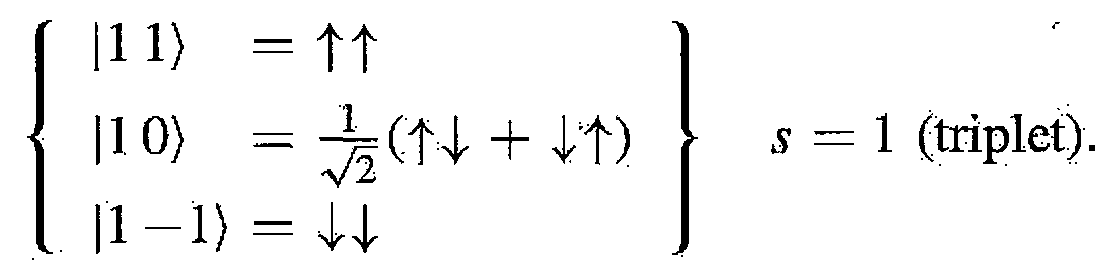
\includegraphics[keepaspectratio, width=0.6\textwidth]{triplet} \end{center}
\item This makes $s=1$ a triplet state
\end{itemize}
}

\frame{
\frametitle{Singlet State}
\begin{itemize}
\item On the contrary, if we look at $s=0$ we have only
\begin{center} 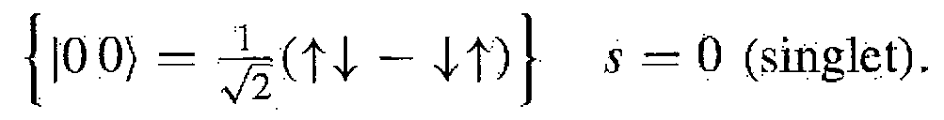
\includegraphics[keepaspectratio, width=0.6\textwidth]{singlet} \end{center}
\item This makes $s=0$ a singlet state
\item If we apply the raising or lowering operator to this we obtain zero
\item Then, the total spin that two spin-1/2 particles can carry is either 1 or 0
\item This is true if the triplet states are eigenvectors of $S^2$ with eigen value $2\hbar^2$
\item The singlet state must also be an eigenvector of $S^2$ with eigenvalue of 0
\end{itemize}
}

\frame{
\frametitle{Spin State Eigenvectors}
\begin{itemize}
\item Let's check:
\begin{equation}
spinsquared S^2 = (S^{(1)} + S^{(2)}) \cdot (S^{(1)} + S^{(2)}) = (S^{(1)})^2 + (S^{(2)})^2 + 2S^{(1)} \cdot S^{(2)}
\end{equation}
\item From previous equations we have
\begin{align*}S^{(1)} \cdot S^{(2)} (\uparrow \downarrow) &= (S_x^{(1)} \uparrow)(S_x^{(2)} \downarrow) + (S_y^{(1)} \uparrow)(S_y^{(2)} \downarrow) + (S_z^{(1)} \uparrow)(S_z^{(2)} \downarrow) \\
&= (\frac{\hbar}{2} \downarrow)(\frac{\hbar}{2} \uparrow) + (\frac{\imath\hbar}{2} \downarrow)(\frac{-\imath\hbar}{2} \uparrow) + (\frac{\hbar}{2} \uparrow)(\frac{-\hbar}{2} \downarrow) \\
&= \frac{\hbar^2}{4}(2 \downarrow \uparrow - \uparrow \downarrow)
\end{align*}
\item As we might expect, the opposite orientation gives:
\begin{displaymath}
S^{(1)} \cdot S^{(2)} (\downarrow \uparrow) = \frac{\hbar^2}{4}(2 \uparrow \downarrow - \downarrow \uparrow)
\end{displaymath}
\end{itemize}
}

\frame{
\frametitle{Proof Continued}
\begin{itemize}
\item If we check:
\begin{displaymath}
S^{(1)} \cdot S^{(2)} |1 0 \rangle = \frac{\hbar^2}{4}\frac{1}{\sqrt{2}}(2 \downarrow\uparrow - \uparrow \downarrow + 2 \ua \da - \da \ua) = \frac{\hbar^2}{4} | 1 0 \rangle
\end{displaymath}
and
\begin{displaymath}
S^{(1)} \cdot S^{(2)} |0 0 \rangle = \frac{\hbar^2}{4}\frac{1}{\sqrt{2}}(2 \da \ua - \ua \da - 2 \ua \da + \da \ua) = - \frac{3\hbar^2}{4} | 0 0 \rangle
\end{displaymath}
\item Then from \ref{spinsquared} we conclude that
\begin{displaymath}
S^2 | 1 0 \rangle = \left( \frac{3\hbar^2}{4} + \frac{3\hbar^2}{4} + 2\frac{\hbar^2}{4} \right) | 1 0 \rangle = 2\hbar^2 | 1 0 \rangle
\end{displaymath}
and
\begin{displaymath}
S^2 | 0 0 \rangle = \left( \frac{3\hbar^2}{4} + \frac{3\hbar^2}{4} + 2\frac{3\hbar^2}{4} \right) | 0 0 \rangle = 0
\end{displaymath}
\end{itemize}
}

\frame{
\frametitle{Spin State Eigenvectors}
\begin{itemize}
\item We have just shown that if you combine spin 1/2 with spin 1/2 you will obtain spin 1 and 0 states.
\item Spin 1 state is an eigenvector of $S^2$ with eigenvalue $2\hbar^2$ and spin 0 state is an eigenvector of $S^2$ with eigenvalue $0$.
\item If we are to expand this to the general case we see that by combing spin $s_1$ with spin $s_2$, we get a total spin of
\begin{displaymath}
s = (s_1 + s_2 ), (s_1 + s_2 - 1), (s_1 + s_2 - 2), ... , |s_1 - s_2 |
\end{displaymath}
\item This gives rise to the combined state of total spin $s$ and $z$-component $m$ as a linear combination of composite states:
\begin{displaymath}
| s m \rangle = \sum_{m_1 + m_2=m} C_{m_1 m_2 m}^{s_1 s_2 s} | s_1 m_1 \rangle | s_2 m_2 \rangle
\end{displaymath}
\end{itemize}
}
 
\frame{
\frametitle{Clebsh-Gordan Table}
\begin{itemize}
\item The Clebsch-Gordan coefficients (a square root sign is present for every entry):
\begin{center} 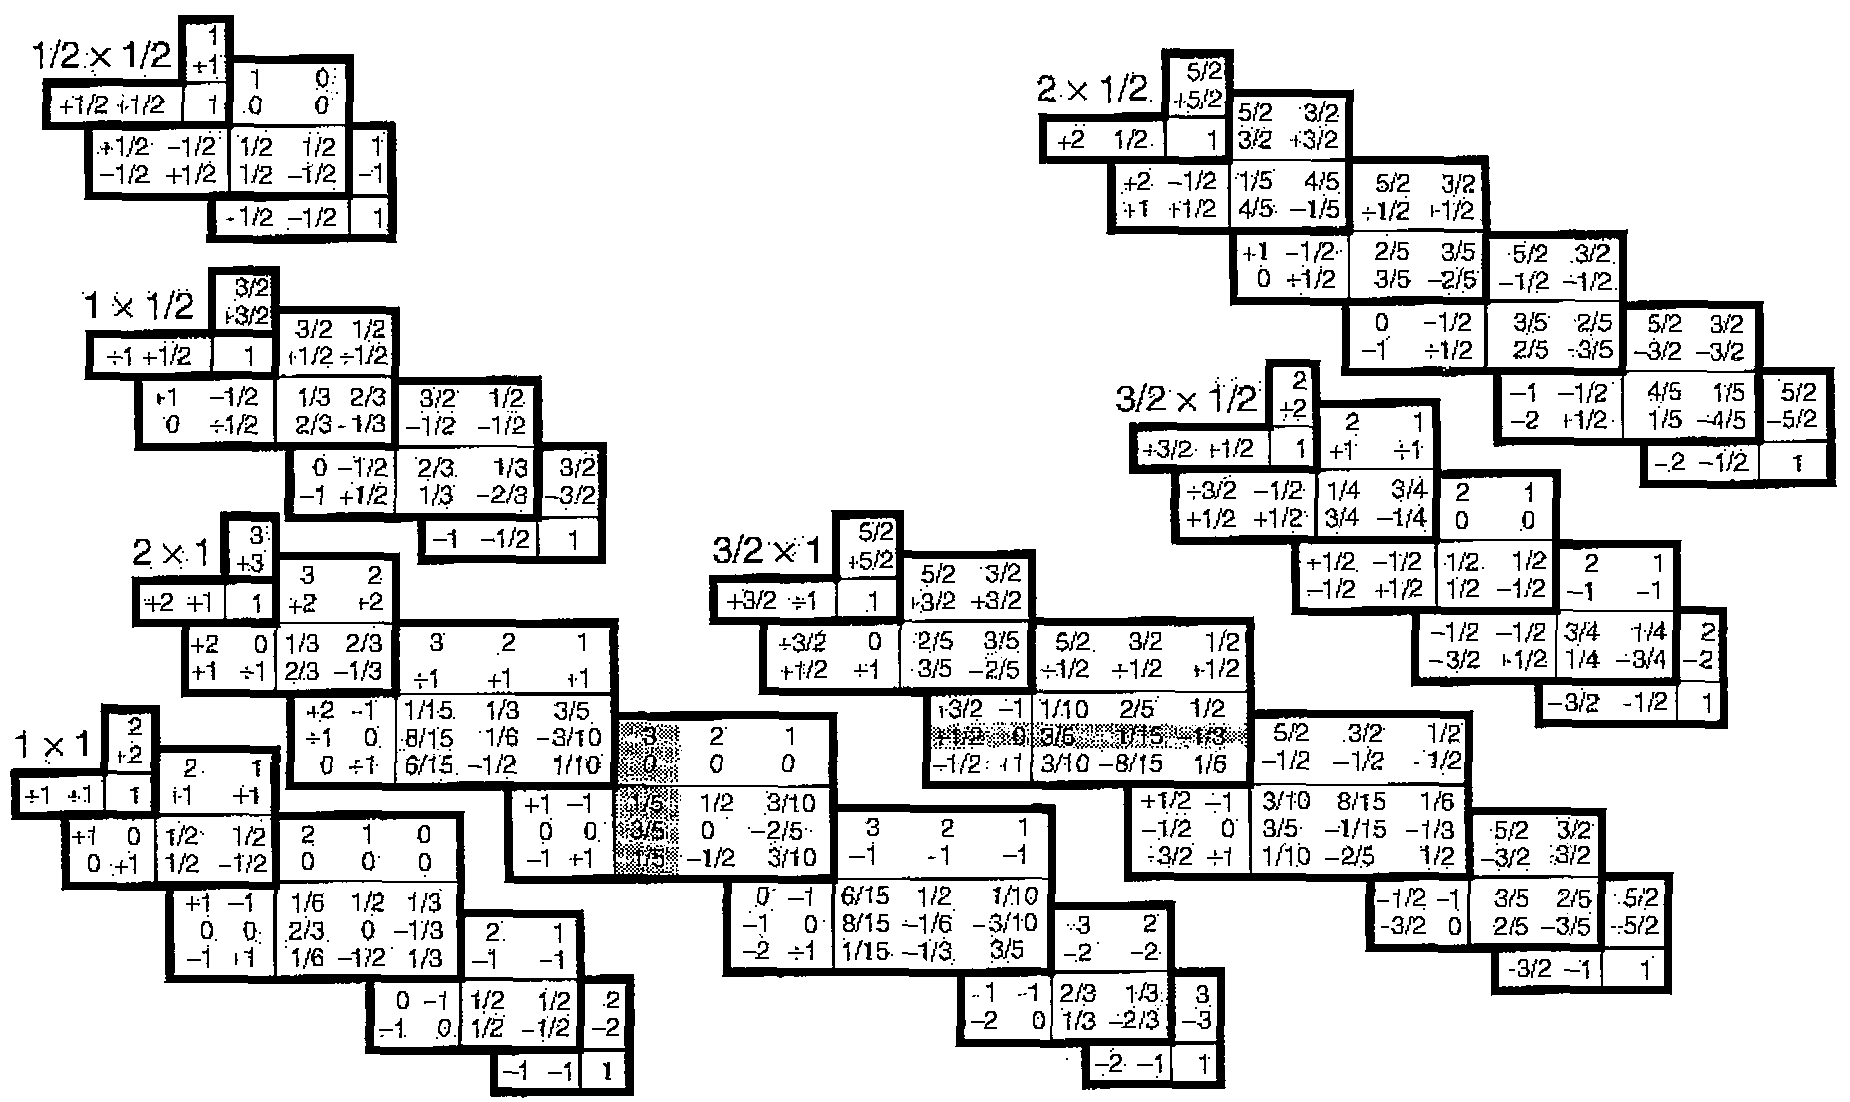
\includegraphics[keepaspectratio, width=.8\textwidth]{clebshgordan} \end{center}
%\ba{| 3 0 \rangle = \frac{1}{\sqrt{5}} |2 1 \rangle | 1 -1 \rangle + \sqrt{\frac{3}{5}} | 2 0 \rangle | 1 0 \rangle + \frac{1}{\sqrt{5}} | 2 -1 \rangle | 1 1 \rangle}
\end{itemize}
}
 
\frame{
\begin{displaymath}
| 3 0 \rangle = \frac{1}{\sqrt{5}} |2 1 \rangle | 1 -1 \rangle + \sqrt{\frac{3}{5}} | 2 0 \rangle | 1 0 \rangle + \frac{1}{\sqrt{5}} | 2 -1 \rangle | 1 1 \rangle
\end{displaymath}
\begin{center} 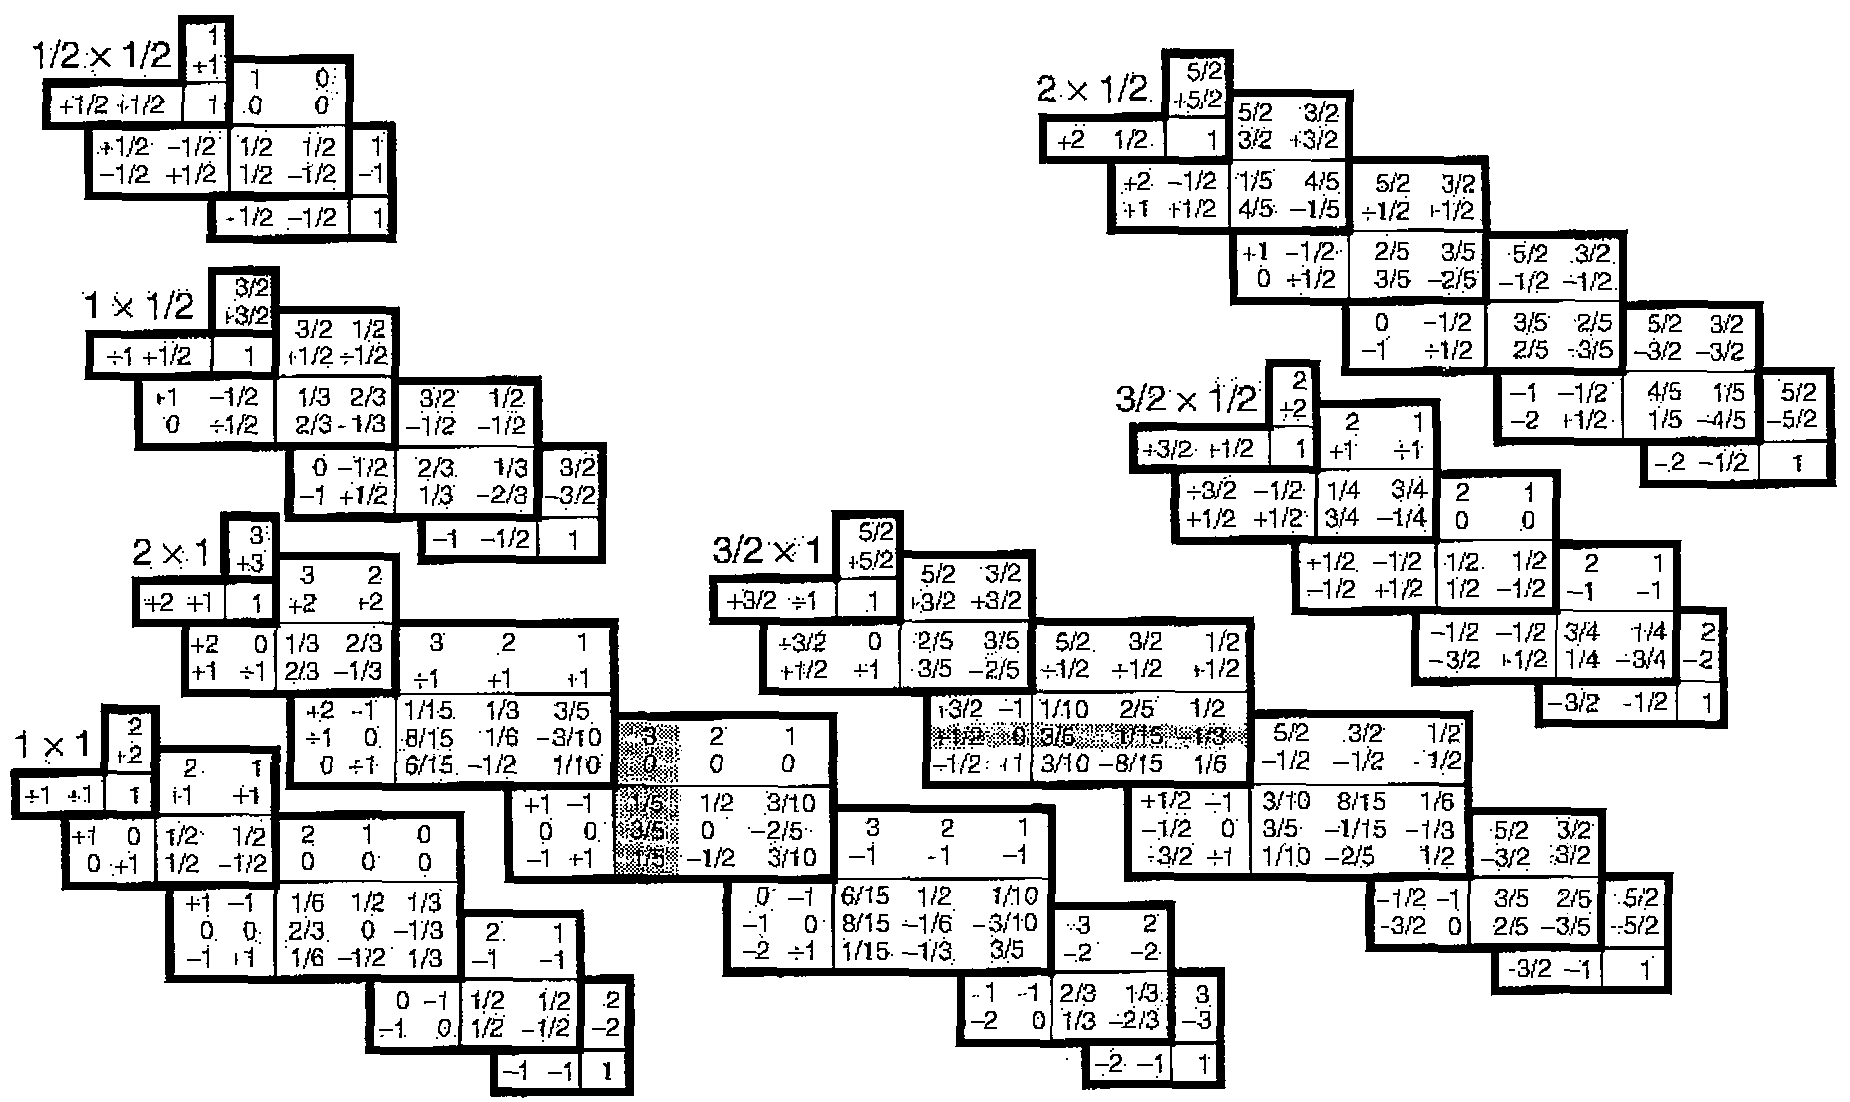
\includegraphics[keepaspectratio, width=.8\textwidth]{clebshgordan} \end{center}
}
 
\begin{frame}
\frametitle{The End}
Thanks for listening!
\end{frame}

\end{document}

\end{document}
